\documentclass[border=10pt]{standalone}
\usepackage{tikz}\usepackage{amsmath}\usetikzlibrary{arrows.meta}
\begin{document}
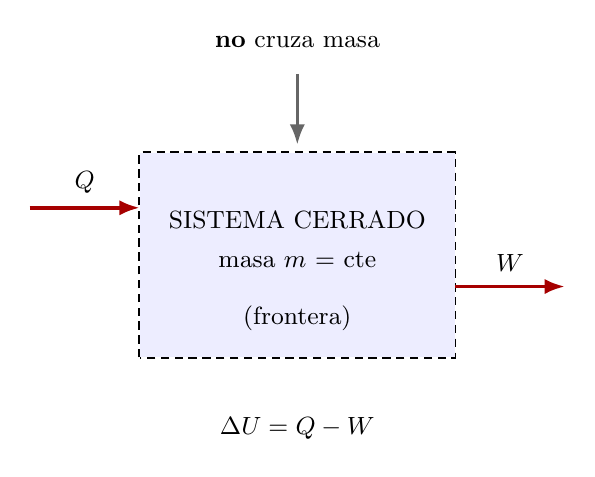
\begin{tikzpicture}[line width=1pt,>={Latex[length=2.6mm]}]
  % frontera (linea discontinua)
  \draw[densely dashed,line width=1.2pt] (0,0) rectangle (4,2.6);
  \fill[blue!7] (0,0) rectangle (4,2.6);
  \node[align=center] at (2,1.5){\small SISTEMA CERRADO\\[2pt]\small masa $m$ = cte};
  \node at (2,0.5){\small (frontera)};
  % calor entra
  \draw[->,red!65!black,line width=1.4pt] (-1.4,1.9)--(0,1.9); \node[above] at (-0.7,1.95){\small $Q$};
  % trabajo sale
  \draw[->,red!65!black,line width=1.4pt] (4,0.9)--(5.4,0.9); \node[above] at (4.7,0.95){\small $W$};
  % masa NO cruza
  \draw[->,black!60,line width=1.2pt] (2,3.6)--(2,2.7); \node[align=center] at (2,4.0){\small \textbf{no} cruza masa};
  \node at (2,-0.9){\small $\Delta U = Q - W$};
\end{tikzpicture}
\end{document}
